\documentclass{beamer}
\usepackage{xcolor} 
\usepackage[utf8]{inputenc}
\usetheme{Madrid}
\usecolortheme{beaver}

%Information to be included in the title page:
\title[About Beamer] %optional
{Software for embedded systems}

\subtitle{Verification Lab.\\ (simple platform - overview)}

\author{Alessandro Danese}
\institute{University of Verona, Verona, Italy\\alessandro.danese@univr.it}
%\date{2019}
 
 
\begin{document}
 
\frame{\titlepage}
 

%==================================================================================
\begin{frame}
\frametitle{Case study: the simple platform}
\centering
Overview of the case study used in SSE Verification Lab\\~\\
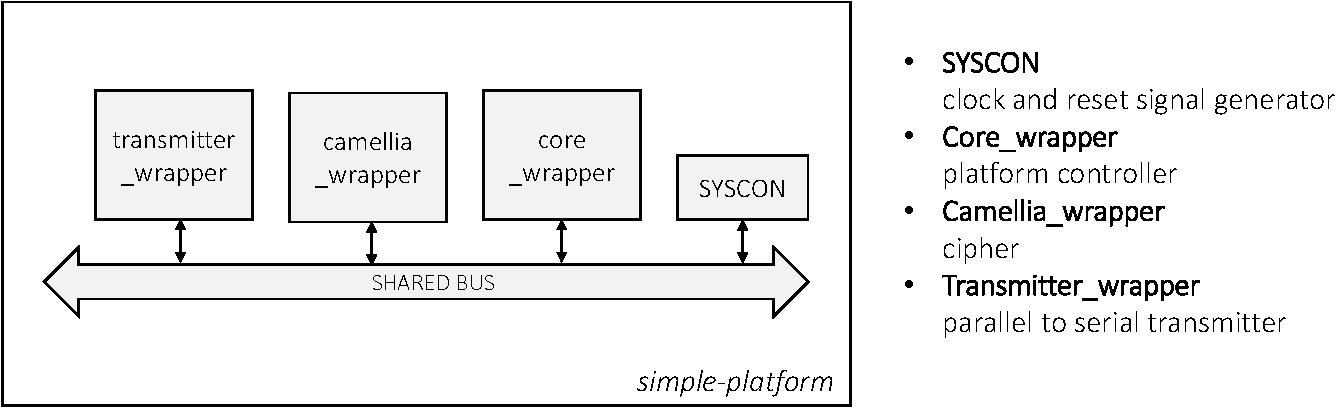
\includegraphics[width=1\columnwidth]{figures/platform-overview-crop.pdf}
\end{frame}
%----------------------------------------------------------------------------------
 
%==================================================================================
\begin{frame}
\frametitle{SYSCON}
The SYSCON component generates the clock signal and the reset signal, 
for all platform's complements.\\~\\

\begin{figure}
	\centering
	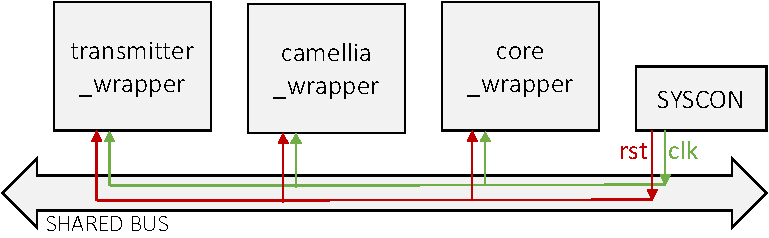
\includegraphics[width=0.9\columnwidth]{figures/syscon-crop.pdf}
\end{figure}

\end{frame}
%----------------------------------------------------------------------------------

%==================================================================================
\begin{frame}

\frametitle{core\_wrapper}
The core\_wrapper component is an abstraction of a RTL CPU executing a firmware.
The firmware code, which is usually stored in memory, is compiled and executed together
with the platform (see next slides).

\begin{figure}
	\centering
	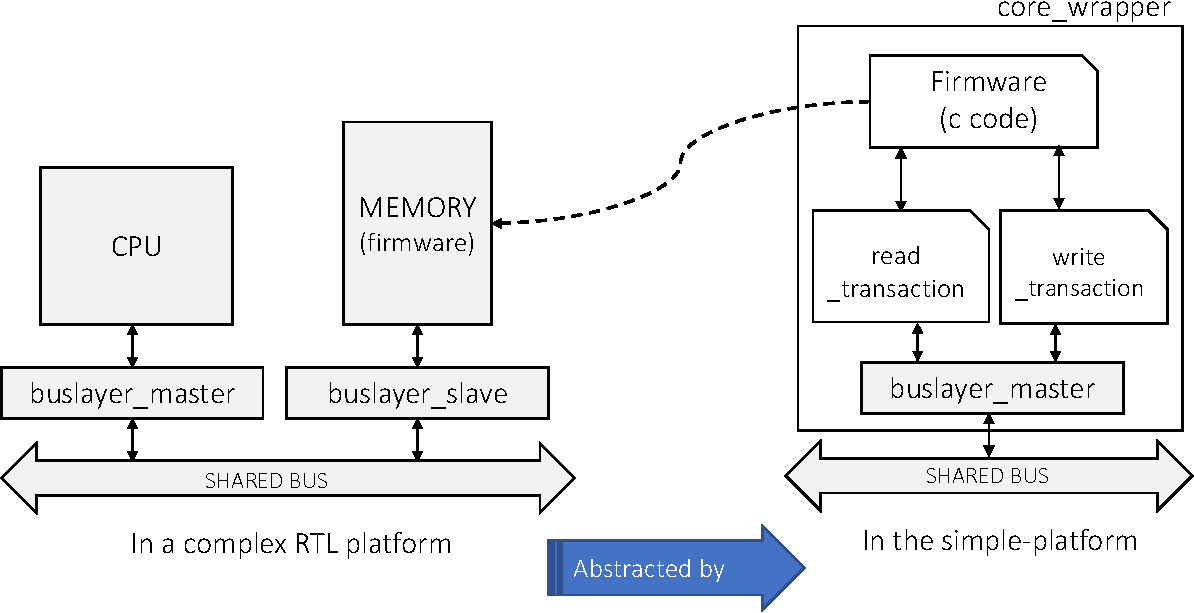
\includegraphics[width=0.9\columnwidth]{figures/cpu_abstraction-crop.pdf}
\end{figure}
\end{frame}
%----------------------------------------------------------------------------------


%==================================================================================
\begin{frame}

\frametitle{read\_transaction}
The core\_wrapper, which behaves as a transactor, provides the following two Verilog
tasks to interact with the platform's components:\\~\\

The read\_transaction provides the reading functionality.
\begin{block}{}
	\textcolor{blue}{task} read\_transaction
	(\textcolor{blue}{input int} addressIn, \textcolor{blue}{input int} byteSelIn, 
	\textcolor{blue}{output int} dataOut, \textcolor{blue}{output byte} errorOut);
\end{block}

\begin{itemize}
	\item \textbf{addresIn}: the address of the component in the platform
	\item \textbf{byteSelIn}: in which byte the component has to provide valid
	                          data  (considering a 4-byte word)
	\item \textbf{dataOut}: the data returned by the addressed component
	\item \textbf{errorOut}: 1 if the write transaction fails, 0 otherwise
\end{itemize}

\end{frame}
%----------------------------------------------------------------------------------

%==================================================================================
\begin{frame}

\frametitle{write\_transaction}

The write\_transaction provides the writing functionality.

\begin{block}{}
	\textcolor{blue}{task} write\_transaction
	(\textcolor{blue}{input int} addressIn, \textcolor{blue}{input int} dataIn,
	\textcolor{blue}{input int} byteSelIn, \textcolor{blue}{output byte} errorOut);
\end{block}

\begin{itemize}
	\item \textbf{addresIn}: the address of the component
	\item \textbf{dataIn}: the data sent to the addressed component
	\item \textbf{byteSelIn}: which byte of dataIn is valid
	\item \textbf{errorOut}: 1 if the read transaction fails, 0 otherwise
\end{itemize}

\end{frame}
%----------------------------------------------------------------------------------

%==================================================================================
\begin{frame}

\frametitle{Exporting Verilog tasks as C methods}

Both Verilog tasks are exported as \textbf{DPI-C} task.
A header file (\textit{vc\_hdrs.h}) including a C method declaration of 
\textit{write\_transaction} and \textit{read\_transaction} is generated by 
the Verilog compiler.

\begin{figure}
	\centering
	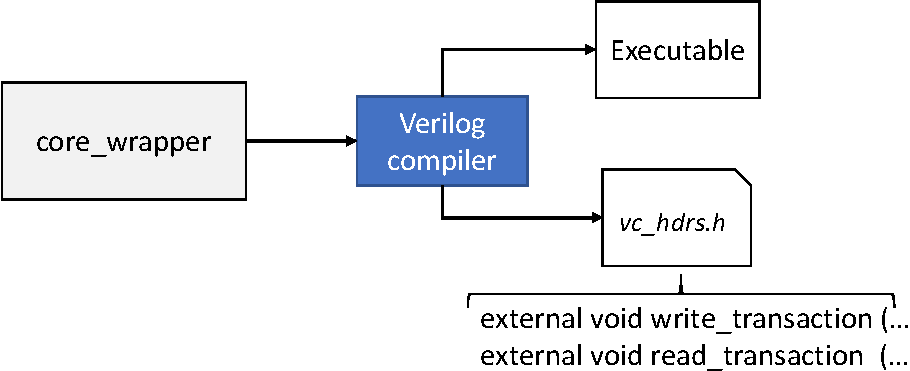
\includegraphics[width=0.7\columnwidth]{figures/vc_hdrs_file-crop.pdf}
\end{figure}

\end{frame}
%----------------------------------------------------------------------------------

%==================================================================================
\begin{frame}

\frametitle{Read/write a memory-mapped component}

The same firmware running in a CPU can be executed in the \textit{simple-platform}
by replacing any operation involving a memory-mapped component with a C-method
call, which corresponds to a Verilog task invocation.

\begin{figure}
	\centering
	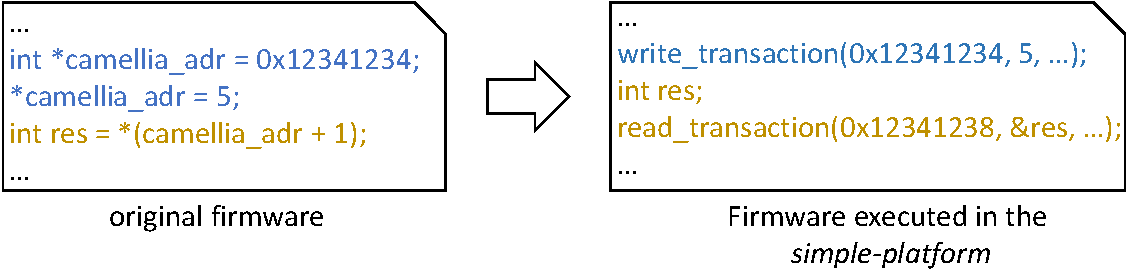
\includegraphics[width=0.9\columnwidth]{figures/firmware-crop.pdf}
\end{figure}

\end{frame}
%----------------------------------------------------------------------------------


%==================================================================================
\begin{frame}

\frametitle{Combining C and Verilog code}

Overview of the C-Verilog compilation flow in the \textit{simple-platform}

\begin{figure}
	\centering
	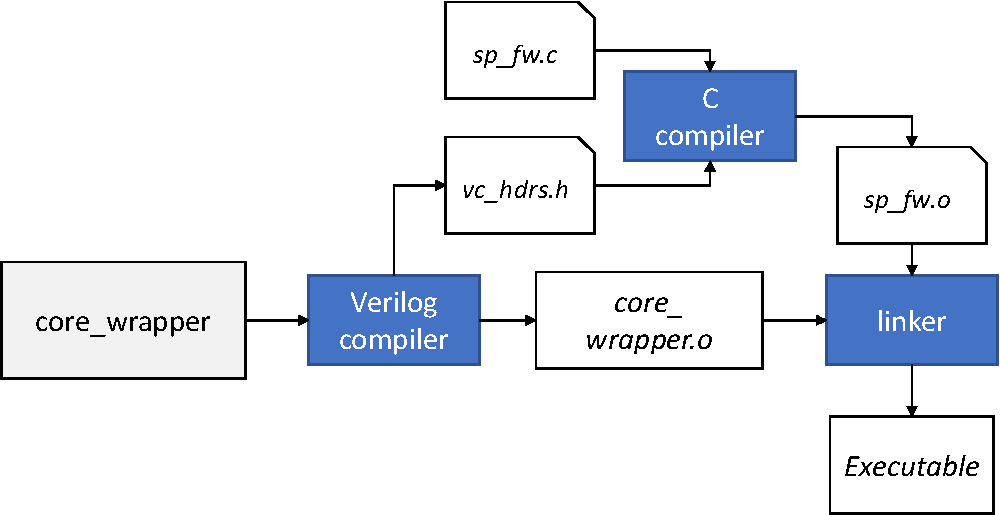
\includegraphics[width=0.9\columnwidth]{figures/c_verilog_flow-crop.pdf}
\end{figure}

\end{frame}
%----------------------------------------------------------------------------------



%==================================================================================
\begin{frame}
\frametitle{buslayer\_master}
The buslayer\_master is the component in charge of forwarding any read/write request
coming from the firmware to the shared bus. \underline{Any transaction} follows the
wishbone protocol rules in the shared bus.
 
\begin{figure}
	\centering
	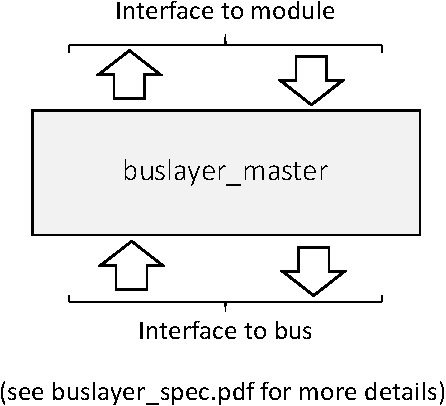
\includegraphics[width=0.4\columnwidth]{figures/buslayer_master-crop.pdf}
\end{figure}

\end{frame}
%----------------------------------------------------------------------------------

%==================================================================================
\begin{frame}
\frametitle{buslayer\_slave}
The buslayer\_slave is the component in charge of forwarding any read/write request
coming from the shared bus to a component. 
The camellia\_wrapper and the serial\_transmitter\_wrapper use a buslayer\_slave to
forward read/write transactions from the shared bus to registers and ports. 

\begin{figure}
	\centering
	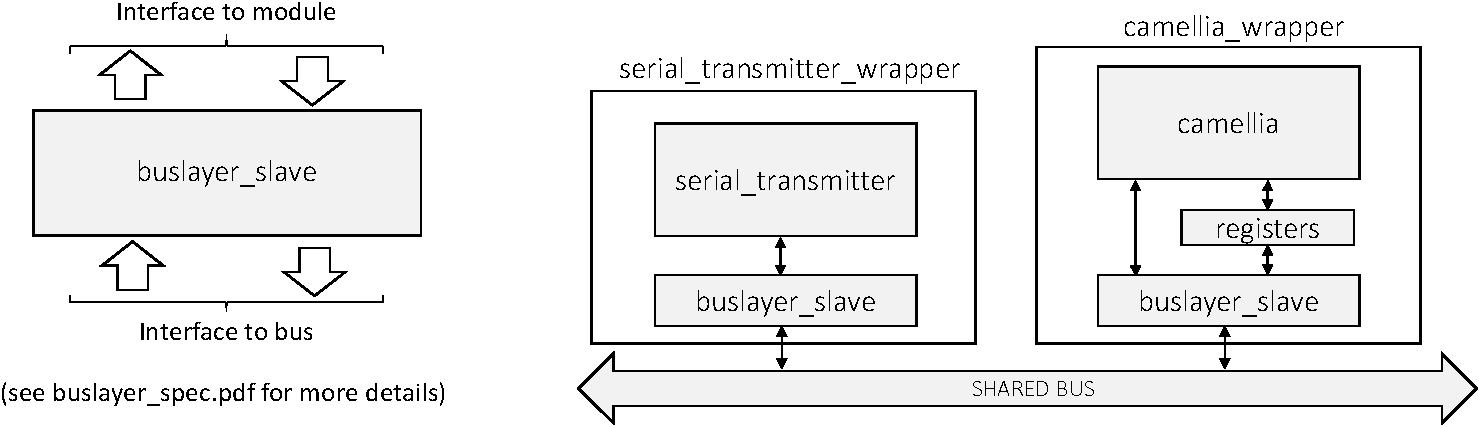
\includegraphics[width=0.9\columnwidth]{figures/buslayer_slave-crop.pdf}
\end{figure}


\end{frame}
%----------------------------------------------------------------------------------

%==================================================================================
\begin{frame}

\frametitle{Memory-mapped components}
The \textit{simple-platform} has a cipher (camellia) and a serial-transmitter.
The two components are memory mapper according to the following address-space map:

\begin{figure}
	\centering
	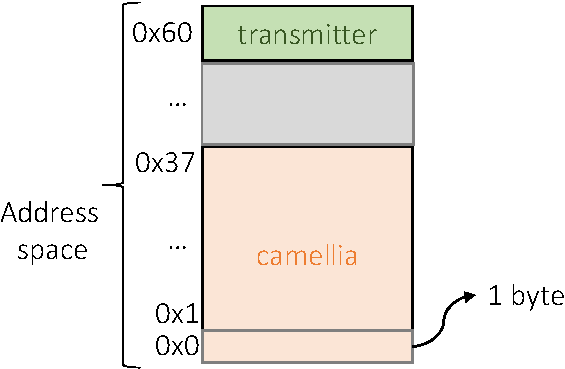
\includegraphics[width=0.5\columnwidth]{figures/address_space-crop.pdf}
\end{figure}

The input port of the serial-transmitter is memory-mapped at the 
\underline{write-only} address 0x60.

\end{frame}
%----------------------------------------------------------------------------------

%==================================================================================
\begin{frame}

\frametitle{Memory-mapped Camellia}
The input/output ports of Camellia are memory-mapped according to the 
address-space map below reported. 
The memory addresses from 0x0 to 0x23 can be read and written. Meanwhile, the addresses
from 0x24 to 0x37 are read-only. \underline{The memory space of Camellia has granularity a word}.

\begin{figure}
	\centering
	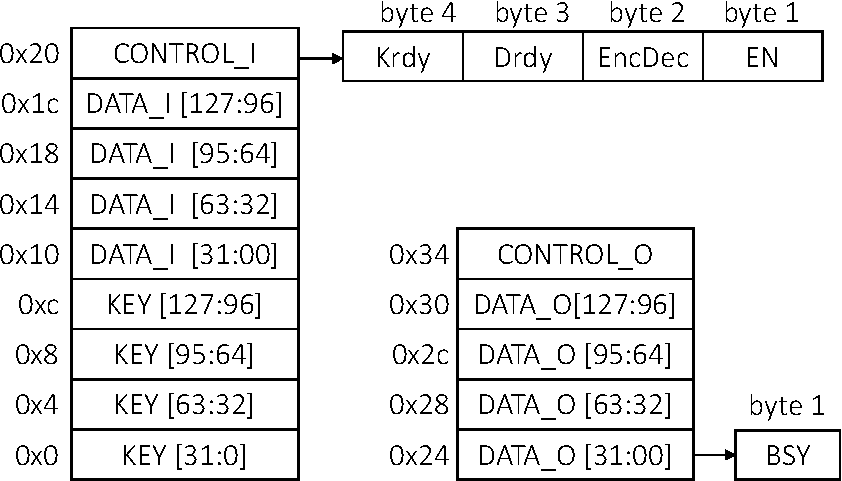
\includegraphics[width=0.65\columnwidth]{figures/camellia-crop.pdf}
\end{figure}

\end{frame}
%----------------------------------------------------------------------------------


%\begin{frame}
%\frametitle{Sample frame title}
%
%In this slide, some important text will be
%\alert{highlighted} beause it's important.
%Please, don't abuse it.
%
%\begin{block}{Remark}
%	Sample text
%\end{block}
%
%\begin{alertblock}{Important theorem}
%	Sample text in red box
%\end{alertblock}
%
%\begin{examples}
%	Sample text in green box. "Examples" is fixed as block title.
%\end{examples}
%\end{frame}

\end{document}